\documentclass[conference]{IEEEtran}

\usepackage{cite}
\usepackage{amsmath,amssymb}
\usepackage{graphicx}
\usepackage{booktabs}
\usepackage{url}
\usepackage{algorithm}
\usepackage{algpseudocode}
\usepackage{placeins}

\graphicspath{{figures/}}
\DeclareMathOperator*{\argmax}{arg\,max}
\newcommand{\Lmax}{L_{\max}}
\newcommand{\Cmax}{C_{\max}}
\newcommand{\Rmin}{R_{\min}}
% Let floats use more of a page, so they stay near their text.
\renewcommand{\topfraction}{0.9}
\renewcommand{\dbltopfraction}{0.9}
\renewcommand{\textfraction}{0.07}
\renewcommand{\floatpagefraction}{0.8}
\renewcommand{\dblfloatpagefraction}{0.8}
\setcounter{topnumber}{3}

\begin{document}

\title{QoS-Aware Service Composition under Latency, Cost and Reliability Constraints}

\author{\IEEEauthorblockN{Aishwary Vansh}
\IEEEauthorblockA{\textit{Dept. of Computer Science and Engineering}\\
\textit{Indian Institute of Information Technology Sri City}\\
Sri City, India}
\and
\IEEEauthorblockN{Soham Biswas}
\IEEEauthorblockA{\textit{Dept. of Computer Science and Engineering}\\
\textit{Indian Institute of Information Technology Sri City}\\
Sri City, India}
}

\maketitle

\begin{abstract}
A composite cloud service must meet end-to-end limits on latency, cost and reliability at the same time. We model candidate services as QoS vectors taken from two real datasets, QWS~2.0 and WS-DREAM, with cost assigned from public cloud prices. On these vectors we implement a greedy composer with constraint-aware repair and a genetic algorithm (GA). We compare their success rate and solution quality as the constraints tighten, measuring quality against the exact optimum from an integer program. Tightness is expressed relative to the feasibility limit of each instance. Over 4,920 problem instances (2,460 per dataset), both composers met all three constraints in every instance up to 98\% of that limit, within 0.023\% of the optimum in the main sweeps ($\rho\le0.98$). At the limit itself, Greedy-Repair succeeded in 63\% of instances on both datasets, against 70--83\% for the GA and 80--90\% for a GA seeded with the greedy result. Greedy-Repair ran in under 1\,ms, about 100 times faster than the GA. A single constraint never binds (its critical tightness is 1 by construction), and the all-three limit (0.904 on QWS, 0.962 on WS-DREAM) lies below every pair's, so the difficulty comes from combining constraints.
\end{abstract}

\begin{IEEEkeywords}
QoS-aware service composition, cloud services, genetic algorithm, greedy algorithm, multi-constraint optimization, QWS, WS-DREAM
\end{IEEEkeywords}

\section{Introduction}
Cloud applications are increasingly built by chaining independent services. A workflow such as \emph{authenticate, fetch, process, store, notify} has one abstract task per step, and each task can be served by several functionally equivalent services that differ in Quality of Service (QoS). The composition problem is to select one candidate per task so that the whole workflow meets the end-to-end requirements of the user~\cite{sheng2014,jula2014}.

\textbf{Research problem.} Composite cloud services must satisfy multiple QoS constraints simultaneously. The attributes conflict: the fastest and most reliable services are usually the most expensive. The search space also grows exponentially, so 10 tasks with 20 candidates each already allow about $10^{13}$ compositions.

\textbf{Research gap.} Student implementations of multi-constraint composition that handle latency, cost and reliability together are still limited. Such implementations seldom use real QoS data, measure results against a proven optimum, or vary constraint tightness in a controlled way.

\textbf{Proposed solution.} We model a set of candidate services with QoS vectors, implement a greedy and a GA-based composer, and compare their success rate and solution quality under different constraint tightness. Our contributions are:
\begin{itemize}
\item an open Python implementation that enforces latency, cost and reliability jointly, with a greedy composer that adds constraint-aware repair and a GA, both evaluated against an exact integer program;
\item an evaluation on two real QoS datasets, QWS~2.0~\cite{almasri2007,almasri2008} and WS-DREAM~\cite{zheng2014}, with cost assigned from public cloud prices;
\item a \emph{relative tightness} measure based on the feasibility limit of each instance, which places the comparison where the constraints actually bind;
\item evidence on both datasets that a single constraint alone never binds, and that the all-three limit (0.904 and 0.962) lies below every pair's limit, so the difficulty comes from combining constraints;
\end{itemize}

\section{Related Work}\label{sec:related}
Surveys by Sheng \emph{et al.}~\cite{sheng2014} and Jula \emph{et al.}~\cite{jula2014} show that QoS-aware selection is a central theme of service composition research.

\textbf{Exact methods.} Zeng \emph{et al.}~\cite{zeng2004} compared local selection, which optimizes each task independently, with global planning by integer programming. Local selection cannot enforce end-to-end constraints, while global planning can but scales poorly. Ardagna and Pernici~\cite{ardagna2007} extended optimization-based selection to adaptive, flexible processes. Our MILP follows this line, but serves as a quality reference.

\textbf{Heuristics.} Yu \emph{et al.}~\cite{yu2007} studied efficient selection algorithms for end-to-end QoS constraints. Alrifai and Risse~\cite{alrifai2009} decomposed global constraints into local ones by integer programming, then applied fast local selection. Our Greedy-Repair starts from the local choice and repairs violations with single swaps, using no solver.

\textbf{Evolutionary methods.} Canfora \emph{et al.}~\cite{canfora2005} showed that a GA is a practical alternative to integer programming for composition. Deb~\cite{deb2000} proposed parameter-free feasibility rules for constraint handling in GAs, which we compare with static penalties.

\textbf{Real QoS data.} QWS~\cite{almasri2007,almasri2008} and WS-DREAM~\cite{zheng2014} are the most widely used public collections of measured web-service QoS. Neither records a price, so studies commonly generate cost; we instead derive it from a public price list.

\section{Problem Formulation}\label{sec:problem}

\subsection{Service and Composition Model}
A workflow has $N$ abstract tasks executed in sequence. Each task $i$ has $M$ candidates, and candidate $j$ has a QoS vector $q_{ij} = (l_{ij}, c_{ij}, r_{ij})$ of latency, cost and reliability. A composition is a vector $a = (a_1,\dots,a_N)$, where $a_i$ is the candidate chosen for task $i$, so there are $M^N$ compositions. End-to-end QoS is
\begin{equation}
L(a) = \sum_{i=1}^{N} l_{i a_i},\quad
C(a) = \sum_{i=1}^{N} c_{i a_i},\quad
R(a) = \prod_{i=1}^{N} r_{i a_i}.
\end{equation}
With $\log R(a) = \sum_i \log r_{i a_i}$, all three aggregates are additive over tasks.

\subsection{Objective and Constraints}
The best and worst aggregate of each attribute come from optimizing that attribute alone, for example $L^{b} = \sum_i \min_j l_{ij}$ and $L^{w} = \sum_i \max_j l_{ij}$. The bounds $C^{b}, C^{w}$ and $\log R^{b}, \log R^{w}$ follow in the same way. Each aggregate is normalized to $[0,1]$, with 1 the best value:
\begin{equation}
\hat L = \frac{L^{w}-L(a)}{L^{w}-L^{b}},\qquad
\hat C = \frac{C^{w}-C(a)}{C^{w}-C^{b}},
\end{equation}
\begin{equation}
\hat R = \frac{\log R(a)-\log R^{w}}{\log R^{b}-\log R^{w}}.
\end{equation}
The objective is a Simple Additive Weighting utility with $w_L+w_C+w_R=1$:
\begin{equation}
U(a) = w_L\hat L + w_C\hat C + w_R\hat R.
\end{equation}
Because every aggregate is additive, $U$ splits exactly into per-service terms, $U(a)=\sum_i u_{i a_i}$. The problem is
\begin{equation}
\max_{a}\; U(a) \;\;\text{s.t.}\;\; L(a)\le \Lmax,\; C(a)\le \Cmax,\; R(a)\ge \Rmin.
\end{equation}
Constraint violation $V(a)$ sums the normalized excess over each limit, with each excess divided by the same range used in (2) and (3). A composition is feasible when $V(a)=0$, up to a tolerance of $10^{-7}$.

\subsection{Constraint Tightness}
Absolute tightness $\tau\in[0,1]$ places each bound between the worst and best aggregate:
\begin{equation}
\Lmax = L^{b} + (1-\tau)(L^{w}-L^{b}),
\end{equation}
and likewise for $\Cmax$ and, in log space, for $\Rmin$. At $\tau=0$ every composition is feasible. Feasible sets are nested in $\tau$, so each instance has a \emph{critical tightness} $\tau^{*}$: the largest $\tau$ that still admits a feasible composition. We find it by bisection with the exact solver, to within $10^{-3}$. \emph{Relative tightness} is $\rho = \tau / \tau^{*}$; with $\rho\le 1$ every instance is solvable, and $\rho=1$ is the edge of feasibility.

\subsection{Complexity}
Choosing one item from each class under several resource limits is the Multi-choice Multi-dimensional Knapsack Problem, which is NP-hard~\cite{yu2007}. This motivates the heuristics below.

\section{Composition Algorithms}\label{sec:algorithms}
All composers rank solutions by Deb's feasibility rules~\cite{deb2000}: a feasible solution beats an infeasible one, two feasible solutions compare by utility, and two infeasible ones compare by lower violation. Since $U\in[0,1]$, this reduces to the key $\kappa(a)=U(a)$ if $V(a)=0$, and $\kappa(a)=-1-V(a)$ otherwise.

\subsection{Greedy Composers}
\textbf{Greedy-Local} is the baseline. It selects $a_i=\argmax_j u_{ij}$ for each task in $O(NM)$ time, ignoring the constraints.

\textbf{Greedy-Repair} (Algorithm~\ref{alg:greedy}) is our greedy composer. It starts from the local choice. While constraints are violated, it applies the single swap with the largest violation reduction per unit of utility lost, the classic knapsack ratio rule. Once feasible, steepest-ascent hill climbing raises utility while keeping feasibility. A swap changes one term of each sum, so all $NM$ swaps are scored in $O(NM)$ per step, and both loops are capped at $10NM$ steps. Repair can stop at a dead end even when a feasible composition exists.

\begin{algorithm}[t]
\caption{Greedy-Repair}\label{alg:greedy}
\footnotesize
\begin{algorithmic}[1]
\Require QoS matrices, constraints, step limit $T=10NM$
\State $a_i \gets \argmax_j u_{ij}$ for every task $i$
\While{$V(a)>0$ \textbf{and} steps $<T$} \Comment{repair}
  \ForAll{swaps $(i,j)$}
    \State $a' \gets a$ with $a_i$ replaced by $j$
    \State $G_{ij}\gets V(a)-V(a')$;\; $D_{ij}\gets \max(U(a)-U(a'),0)$
  \EndFor
  \If{no swap has $G_{ij}>0$} \textbf{break} \Comment{dead end}
  \EndIf
  \State $(i^{*},j^{*})\gets \argmax_{G_{ij}>0}\; G_{ij}/(D_{ij}+10^{-9})$
  \State $a_{i^{*}} \gets j^{*}$
\EndWhile
\If{$V(a)=0$} \Comment{improve}
  \While{steps $<T$}
    \State find the feasible swap with the largest gain in $U$
    \If{gain $\le 0$} \textbf{break}
    \EndIf
    \State apply that swap
  \EndWhile
\EndIf
\State \Return $a$ and its feasibility status
\end{algorithmic}
\end{algorithm}

\subsection{Genetic Algorithm}
The GA (Algorithm~\ref{alg:ga}) encodes a composition as an integer chromosome of length $N$, so every chromosome is a valid composition. Table~\ref{tab:ga} lists its settings. Fitness is the key $\kappa$ by default; a static-penalty variant uses $U-\lambda V$.

\textbf{GA+Greedy} seeds the initial population with the Greedy-Repair and Greedy-Local results, and the best composition seen is tracked across generations, so the hybrid never returns a composition worse than Greedy-Repair's.

\begin{algorithm}[t]
\caption{Genetic Algorithm Composer}\label{alg:ga}
\footnotesize
\begin{algorithmic}[1]
\Require population $P$, generations $G$, rates $p_c,p_m$, tournament $k$, elites $e$, stagnation limit $s$
\State create $P$ random chromosomes; evaluate $\kappa$
\State (GA+Greedy only) insert the Greedy-Repair and Greedy-Local results
\State $a^{\text{best}} \gets$ individual with the highest $\kappa$
\For{$g=1$ to $G$}
  \State $E\gets$ top $e$ individuals
  \State select parent pairs by tournament of size $k$
  \State with probability $p_c$, apply uniform crossover to a pair
  \State reset each child gene with probability $p_m$ to another candidate
  \State population $\gets E\,\cup$ children; evaluate $\kappa$
  \If{$\kappa$ improved} update $a^{\text{best}}$; reset counter
  \Else\ increment counter
  \EndIf
  \If{counter $\ge s$} \textbf{break}
  \EndIf
\EndFor
\State \Return $a^{\text{best}}$
\end{algorithmic}
\end{algorithm}

\begin{table}[t]
\centering
\caption{GA Settings}\label{tab:ga}
\footnotesize
\begin{tabular}{ll}
\toprule
Parameter & Value \\
\midrule
Population, generations & $P=100$, $G=300$ \\
Selection & Tournament, $k=3$ \\
Crossover, mutation & Uniform $p_c=0.9$; random reset $p_m=1/N$ \\
Elitism, early stop & $e=2$; 80 generations without improvement \\
Constraint handling & Deb's rules (default), or penalty $U-\lambda V$ \\
\bottomrule
\end{tabular}
\end{table}

\subsection{Reference Solvers}
\textbf{Optimal-MILP} solves the 0-1 program with variables $x_{ij}$: maximize $\sum_{ij} u_{ij}x_{ij}$ subject to $\sum_j x_{ij}=1$ for every task and three linear QoS rows, with reliability in log form. All terms are linear, so the model is exact. We solve it with HiGHS~\cite{huangfu2018} through SciPy~\cite{virtanen2020}. It gives the optimum $U^{*}$ (within HiGHS's default relative gap of 0.01\%, so a heuristic can exceed $U^{*}$ by at most that margin, as happened in 20 of over 25,000 runs) and proves infeasibility, and unit tests confirm that it agrees with brute-force enumeration. \textbf{Random} search keeps the best of 30,000 uniform samples, close to the worst-case GA budget of 29,500 evaluations.

\begin{figure*}[t]
\centering
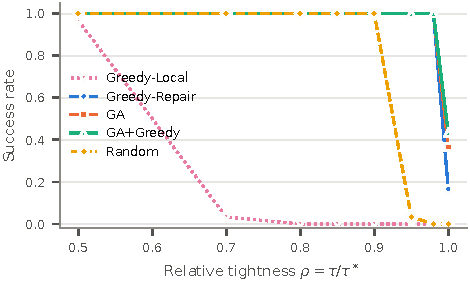
\includegraphics[width=\textwidth]{success_rho}
\caption{Success rate vs relative tightness on (a) QWS 2.0 and (b) WS-DREAM ($N=10$, $M=20$, 30 instances per point; all instances are solvable).}
\label{fig:success}
\end{figure*}

\begin{figure*}[t]
\centering
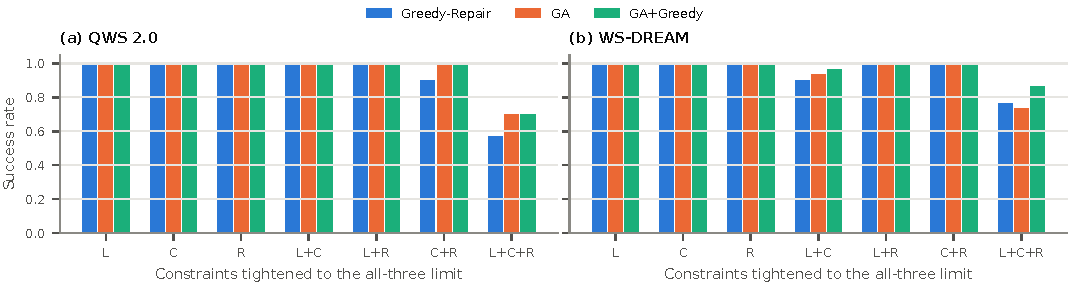
\includegraphics[width=\textwidth]{constraint_combinations}
\caption{Success rate when single constraints, pairs or all three are tightened to the all-three limit $\tau^{*}$, on (a) QWS 2.0 and (b) WS-DREAM.}
\label{fig:combinations}
\end{figure*}

\section{Experimental Setup}\label{sec:setup}

\subsection{Datasets}
Table~\ref{tab:data} summarizes the two real datasets.

\textbf{QWS~2.0}~\cite{almasri2007,almasri2008} contains 2,507 real web services, each with nine QoS attributes averaged over six days of measurement. We use Response Time as latency and Reliability as reliability.

\textbf{WS-DREAM} dataset~1~\cite{zheng2014} contains response times and throughputs measured by 339 users on 5,825 services; invalid invocations are marked $-1$. Each instance is built for one random user, using that user's measured response time. Reliability is the share of users whose invocation returned a valid measurement, an observed success ratio used as a proxy. Services valid for fewer than half of the users are dropped (248 services).

\textbf{Cost.} Neither dataset records a price. Each service is ranked by its measured throughput, an indicator of provisioned capacity. The ranking is split into six equal groups mapped to the AWS EC2 t3 sizes nano to xlarge (on-demand, Linux, us-east-1)~\cite{aws2026}, priced from \$0.0052 to \$0.1664 per hour. The cost of a composition is therefore its hourly hosting cost. This yields a genuine trade-off: higher-priced services have lower latency (Spearman $-0.35$ on QWS and $-0.54$ on WS-DREAM).

\textbf{Instances.} $N\times M$ distinct services are drawn without replacement and split at random into $N$ tasks, since neither dataset labels service functions. Weights are equal, $w_L=w_C=w_R=1/3$.

\begin{table}[t]
\centering
\caption{QoS Data Used}\label{tab:data}
\footnotesize
\begin{tabular}{lll}
\toprule
 & QWS 2.0 & WS-DREAM \\
\midrule
Services used & 2,507 & 5,577 \\
Latency (median) & 227\,ms & 345\,ms (per service) \\
Latency source & Measured & Measured, per user \\
Reliability range & 0.33--0.89 & 0.50--1.00 \\
Reliability source & Measured & Success ratio \\
Cost & \multicolumn{2}{l}{EC2 t3 price by throughput tier} \\
\bottomrule
\end{tabular}
\end{table}

\subsection{Tool Choice and Implementation}
We used a custom Python model rather than CloudSim~\cite{calheiros2011}, as the problem statement permits. CloudSim simulates data-center resources, whereas this problem is a selection over known QoS values. A custom model also allows the exact solver and thousands of repeated runs. Each composition is an integer vector, and the GA evaluates a whole generation as one array operation. All randomness is seeded, the datasets are downloaded and checked by md5 sum, and 73 unit tests validate the model, the solvers and the data loaders.

\subsection{Metrics and Experiments}
\emph{Success rate} is the share of solvable instances for which a composer returns a feasible composition. \emph{Optimality gap} is $(U^{*}-U)/U^{*}$ over successful runs. \emph{Runtime} is the wall-clock time per instance.

Each setting uses 30 instances with fixed seeds (2,460 per dataset, including the sweeps below). The default size is $N=10$, $M=20$. We sweep absolute $\tau$ (12 levels) and relative $\rho$ (8 levels); scale $N\in\{5,10,20,40\}$ and $M\in\{10,20,50,100\}$ at $\rho=0.95$; tighten each single constraint, each pair and all three at $0.9$ and $1.0$ times the all-three limit $\tau^{*}$ (a $1.2$ level would exceed the valid range $[0,1]$ and is clamped to $\tau=1$, where a single constraint is feasible by construction, so we measure each subset's own critical tightness $\tau^{*}_S$ by bisection instead); compare constraint handling; and record GA convergence at $N=20$, $M=30$. The $\rho\in\{0.98,0.99,1.0\}$ band is repeated over 150 instances, and $\rho\in\{0.95,1.0\}$ is repeated with skewed utility weights. We label the experiments E1 (tightness), E2 (tasks), E3 (candidates), E4 (constraint subsets), E5 (handling), E6 (convergence), E7 (whole-dataset), E8 (150-instance limit band) and E9 (weights). E1, E4 and E5 share the same 30 instances, so their comparisons are paired. Paired Wilcoxon signed-rank tests compare quality; their $p$-values are not corrected for multiple comparisons.

\section{Results and Analysis}\label{sec:results}

\subsection{Feasibility Limit}
For $N=10$ and $M=20$, $\tau^{*}$ averaged 0.904 on QWS (0.876--0.926) and 0.962 on WS-DREAM (0.922--0.976). On QWS, all 30 instances were solvable up to $\tau=0.85$ and 20 at $\tau=0.9$. The constraints therefore bind only in a narrow band of high $\tau$, which is why the rest of the evaluation uses $\rho$. No composer ever claimed feasibility on an unsolvable instance.

\subsection{Success Rate vs Tightness}
Fig.~\ref{fig:success} gives the main result. Greedy-Local starts failing at $\rho=0.95$ on QWS and at $\rho=0.98$ on WS-DREAM, because its unconstrained choice breaks the limits. Random search collapses at $\rho=0.95$ on QWS and at $\rho=0.98$ on WS-DREAM. Greedy-Repair, the GA and GA+Greedy keep 100\% success up to $\rho=0.98$ on both datasets. At the feasibility limit $\rho=1$, success is 63\% for Greedy-Repair on both datasets, 70\% and 83\% for the GA, and 90\% and 80\% for GA+Greedy. The hybrid beats Greedy-Repair on 8 instances and loses on none on QWS ($p=0.0078$); on WS-DREAM the result is 5 to 0 ($p=0.063$). The GA's lead over Greedy-Repair is not significant on either dataset ($p=0.77$ and $0.14$).

Because 30 instances give success rates with roughly $\pm$16\,pp confidence intervals, the band $\rho\in\{0.98,0.99,1.0\}$ was repeated over 150 instances (Table~\ref{tab:limit}). Up to $\rho=0.99$ every core composer stays at 97--100\% success on both datasets. At the limit, Greedy-Repair drops to 60\% (QWS) and 72\% (WS-DREAM), the GA to 67\% and 82\%, and GA+Greedy and the mild penalty reach 79\% and 84\%. Paired tests on these 150 instances support the mild penalty's lead over the plain GA on QWS (30 against 14 instances better, $p=0.005$) but not on WS-DREAM (31 against 15, $p=0.13$), while GA+Greedy beats Greedy-Repair on both datasets ($p<10^{-4}$).

\begin{table}[t]
\centering
\caption{Success Rate Near the Limit over 150 Instances (E8). GL = Greedy-Local, GR = Greedy-Repair, G+G = GA+Greedy, $\lambda=1$ = GA with a Static Penalty $\lambda=1$}\label{tab:limit}
\resizebox{\columnwidth}{!}{\begin{tabular}{lcccc}
\toprule
Data & Composer & \multicolumn{3}{c}{Success rate} \\
\cmidrule(lr){3-5}
 & & $\rho=0.98$ & $0.99$ & $1.00$ \\
\midrule
QWS 2.0 & GL & 0.18 & 0.08 & 0.03 \\
 & GR & 1.00 & 0.97 & 0.60 \\
 & GA & 1.00 & 0.99 & 0.67 \\
 & $\lambda=1$ & 1.00 & 1.00 & 0.79 \\
 & G+G & 1.00 & 0.99 & 0.79 \\
\midrule
WS-DREAM & GL & 0.78 & 0.47 & 0.01 \\
 & GR & 1.00 & 1.00 & 0.72 \\
 & GA & 1.00 & 1.00 & 0.82 \\
 & $\lambda=1$ & 1.00 & 1.00 & 0.84 \\
 & G+G & 1.00 & 1.00 & 0.84 \\
\bottomrule
\end{tabular}
}
\end{table}

\subsection{Solution Quality and Runtime}
Table~\ref{tab:gapruntime} shows that the three main composers return the optimum, or a composition within 0.023\% of it, at every level up to $\rho=0.98$. Random search stays 2.7--6.2\% from the optimum while it still succeeds. Greedy-Repair runs in under 1\,ms, compared with 6--14\,ms for the exact solver, 21--31\,ms for GA+Greedy and 28--45\,ms for the GA.

\begin{table}[t]
\centering
\caption{Mean Optimality Gap (\%) and Runtime Range, $N=10$, $M=20$. ``--'' Means Fewer than 5 Successes}\label{tab:gapruntime}
\resizebox{\columnwidth}{!}{\begin{tabular}{llcccc}
\toprule
Dataset & Composer & $\rho=0.90$ & $0.95$ & $0.98$ & Runtime (ms) \\
\midrule
QWS 2.0 & Greedy-Local & 0.000 & 0.000 & 0.000 & 0.1--0.1 \\
 & Greedy-Repair & 0.000 & 0.003 & 0.023 & 0.2--0.5 \\
 & GA & 0.000 & 0.004 & 0.012 & 28.1--37.3 \\
 & GA+Greedy & 0.000 & 0.003 & 0.023 & 21.3--28.4 \\
 & Random & 6.239 & -- & -- & 11.1--12.4 \\
 & Optimal-MILP & 0.000 & 0.000 & 0.000 & 6.1--11.2 \\
\midrule
WS-DREAM & Greedy-Local & 0.000 & 0.000 & 0.000 & 0.1--0.1 \\
 & Greedy-Repair & 0.000 & 0.000 & 0.000 & 0.2--0.4 \\
 & GA & 0.000 & 0.000 & 0.006 & 36.4--44.6 \\
 & GA+Greedy & 0.000 & 0.000 & 0.000 & 26.5--31.3 \\
 & Random & 3.593 & 2.697 & -- & 12.6--16.1 \\
 & Optimal-MILP & 0.000 & 0.000 & 0.000 & 9.0--14.2 \\
\bottomrule
\end{tabular}
}
\end{table}

\subsection{Scalability}
Table~\ref{tab:scale} shows scaling at $\rho=0.95$. Greedy-Repair, the GA and GA+Greedy keep 100\% success at every size on both datasets. Greedy-Local drops to 43\% at $N=40$ on QWS, and Random fails for $N\ge10$ on QWS. Gaps stay below 0.006\% for Greedy-Repair and GA+Greedy and at most 0.03\% for the GA. At $N=40$, Greedy-Repair needs 0.4\,ms on QWS, against 25\,ms for the MILP, 32\,ms for GA+Greedy and 124\,ms for the GA.

\begin{table}[t]
\centering
\caption{Scalability at $\rho=0.95$ (GL and Rnd Success; Gap and Runtime of the Main Composers). GL = Greedy-Local, Rnd = Random}\label{tab:scale}
\resizebox{\columnwidth}{!}{\begin{tabular}{llcccccccc}
\toprule
 & & \multicolumn{2}{c}{Success} & \multicolumn{3}{c}{Gap (\%)} & \multicolumn{3}{c}{Runtime (ms)} \\
\cmidrule(lr){3-4}\cmidrule(lr){5-7}\cmidrule(lr){8-10}
Data & Size & GL & Rnd & GR & GA & G+G & GR & GA & MILP \\
\midrule
QWS 2.0 & $N=5$ & 0.87 & 0.93 & 0.000 & 0.000 & 0.000 & 0.3 & 35.1 & 14.1 \\
 & $N=10$ & 0.57 & 0.00 & 0.000 & 0.012 & 0.000 & 0.3 & 59.2 & 18.6 \\
 & $N=20$ & 0.47 & 0.00 & 0.006 & 0.012 & 0.006 & 0.5 & 90.8 & 25.7 \\
 & $N=40$ & 0.43 & 0.00 & 0.001 & 0.012 & 0.001 & 0.5 & 160.3 & 49.3 \\
 & $M=10$ & 0.67 & 0.13 & 0.000 & 0.007 & 0.000 & 0.3 & 39.7 & 13.5 \\
 & $M=20$ & 0.57 & 0.00 & 0.000 & 0.004 & 0.000 & 0.4 & 57.6 & 18.1 \\
 & $M=50$ & 0.80 & 0.00 & 0.000 & 0.002 & 0.000 & 0.5 & 69.4 & 29.5 \\
 & $M=100$ & 1.00 & 0.00 & 0.000 & 0.030 & 0.000 & 0.3 & 91.2 & 54.8 \\
\midrule
WS-DREAM & $N=5$ & 1.00 & 1.00 & 0.000 & 0.000 & 0.000 & 0.3 & 33.3 & 15.7 \\
 & $N=10$ & 0.97 & 0.90 & 0.000 & 0.000 & 0.000 & 0.3 & 46.8 & 18.1 \\
 & $N=20$ & 1.00 & 0.10 & 0.000 & 0.000 & 0.000 & 0.5 & 73.9 & 24.9 \\
 & $N=40$ & 1.00 & 0.00 & 0.000 & 0.001 & 0.000 & 0.3 & 143.1 & 44.6 \\
 & $M=10$ & 0.93 & 0.73 & 0.000 & 0.000 & 0.000 & 0.3 & 38.1 & 14.6 \\
 & $M=20$ & 1.00 & 0.87 & 0.000 & 0.000 & 0.000 & 0.3 & 45.3 & 18.3 \\
 & $M=50$ & 1.00 & 0.93 & 0.000 & 0.000 & 0.000 & 0.3 & 61.3 & 26.3 \\
 & $M=100$ & 1.00 & 0.93 & 0.000 & 0.016 & 0.000 & 0.3 & 81.3 & 46.4 \\
\bottomrule
\end{tabular}
}
\end{table}

\subsection{Whole-Dataset Instances}
Table~\ref{tab:e7} repeats the sweep with almost the entire dataset inside one problem: 2,500 services as $10\times250$ or $50\times50$ on QWS, and 5,500 as $10\times550$ or $50\times110$ on WS-DREAM. Up to $\rho=0.98$ Greedy-Repair and GA+Greedy still solve every instance and the GA keeps 97--100\% with mean gaps below 0.5\%; at $\rho=1$ success drops for all composers: Greedy-Repair and GA+Greedy reach 63--70\% on QWS and 90\% on WS-DREAM, while the plain GA fails almost everywhere (0--23\%).

\begin{table}[t]
\centering
\caption{Success Rate on Whole-Dataset Instances (E7). G-Repair = Greedy-Repair, G+G = GA+Greedy}\label{tab:e7}
\resizebox{\columnwidth}{!}{\begin{tabular}{lllcccc}
\toprule
Data & Size & Composer & \multicolumn{4}{c}{Success rate} \\
\cmidrule(lr){4-7}
 & & & $\rho=0.90$ & $0.95$ & $0.98$ & $1.00$ \\
\midrule
QWS 2.0 & 10x250 & G-Repair & 1.00 & 1.00 & 1.00 & 0.67 \\
 &  & GA & 1.00 & 1.00 & 0.97 & 0.13 \\
 &  & G+G & 1.00 & 1.00 & 1.00 & 0.70 \\
QWS 2.0 & 50x50 & G-Repair & 1.00 & 1.00 & 1.00 & 0.63 \\
 &  & GA & 1.00 & 1.00 & 1.00 & 0.00 \\
 &  & G+G & 1.00 & 1.00 & 1.00 & 0.63 \\
\midrule
WS-DREAM & 10x550 & G-Repair & 1.00 & 1.00 & 1.00 & 0.90 \\
 &  & GA & 1.00 & 1.00 & 1.00 & 0.23 \\
 &  & G+G & 1.00 & 1.00 & 1.00 & 0.90 \\
WS-DREAM & 50x110 & G-Repair & 1.00 & 1.00 & 1.00 & 0.90 \\
 &  & GA & 1.00 & 1.00 & 1.00 & 0.00 \\
 &  & G+G & 1.00 & 1.00 & 1.00 & 0.90 \\
\bottomrule
\end{tabular}
}
\end{table}

\subsection{Single vs Combined Constraints}
For each constraint subset $S$ we bisect its own critical tightness $\tau^{*}_S$, tightening only the attributes in $S$ and leaving the others at $\tau=0$ (Table~\ref{tab:critical}). A single attribute always reaches $\tau^{*}_S=1$: picking each task's own best service attains that attribute's best aggregate, so a lone constraint can never make the problem infeasible. Hardness comes from combining attributes. Each pair costs 2.9--7.9\,pp of tightness headroom on QWS ($0.971$, $0.963$, $0.921$) and 0.7--3.0\,pp on WS-DREAM ($0.970$, $0.993$, $0.988$), and the all-three limit is below every pair's ($0.904$ and $0.962$). At exactly $\tau^{*}$ (Fig.~\ref{fig:combinations}), all three together is the hardest case for every composer: Greedy-Repair succeeds on 63\% of instances on both datasets, the GA on 70\% and 83\%, and GA+Greedy on 90\% and 80\%, while on every pair Greedy-Repair succeeds on at least 90\% of instances on QWS and on all of them on WS-DREAM, and the GA and GA+Greedy on all of them on both datasets. Greedy-Local fails on different attributes in each dataset, mainly reliability on QWS and latency on WS-DREAM.

\begin{table}[t]
\centering
\caption{Mean Critical Tightness $\tau^{*}_S$ per Constraint Subset (Bisection with the Exact Solver). L = Latency, C = Cost, R = Reliability}\label{tab:critical}
\resizebox{\columnwidth}{!}{\begin{tabular}{lccc}
\toprule
Dataset & L & R & L+R \\
\midrule
QWS 2.0 & 1.000 & 1.000 & 0.963 \\
WS-DREAM & 1.000 & 1.000 & 0.993 \\
\bottomrule
\end{tabular}
}
\end{table}

\subsection{GA Constraint Handling and Convergence}
We also compared Deb's rules with static penalties $\lambda=1,10,100$ on the same 30 instances. All variants reach 100\% at $\rho=0.9$ and $0.95$. At $\rho=1$, Deb's rules reached 70\% (QWS) and 83\% (WS-DREAM), the penalties 80--87\% and 77--90\%, and GA+Greedy 90\% and 80\%. These differences lie within the $\pm$16\,pp interval of 30 runs, and the paired comparison of $\lambda=1$ against Deb's rules is not significant at 30 instances (5 against 3 better instances on QWS, $p=0.45$; 6 against 3 on WS-DREAM, $p=0.51$). Over the 150 instances of E8, however, $\lambda=1$ leads Deb's rules on QWS ($p=0.005$) but not on WS-DREAM ($p=0.13$). We therefore keep Deb's rules as the default and report the mild penalty as an alternative rather than a consistent improvement.

Fig.~\ref{fig:conv} shows convergence at $N=20$, $M=30$, $\rho=0.95$. The plain GA has a feasible solution in all runs by generation 25 on both datasets, reaches a mean $U/U^{*}$ of 0.990 (QWS) and 0.996 (WS-DREAM) by generation 50, and about 1.000 by generation 200. The hybrid starts at the optimum in this setting.

\begin{figure}[t]
\centering
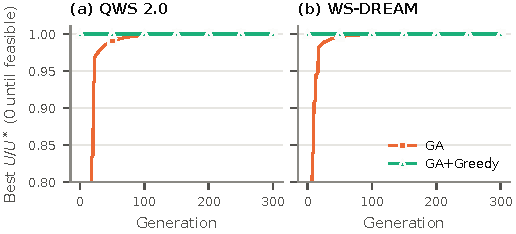
\includegraphics[width=\columnwidth]{convergence}
\caption{GA convergence at $N=20$, $M=30$, $\rho=0.95$, averaged over 30 instances.}
\label{fig:conv}
\end{figure}

\subsection{Utility Weights}
All experiments above use equal weights. Repeating $\rho\in\{0.95,1.0\}$ with one weight raised to $0.6$ (Table~\ref{tab:weights}) moves Greedy-Repair's success at the limit 20\,pp below and 14\,pp above its equal-weight value of 63\% on QWS (43--77\%), because repair follows the utility, not the constraints. GA+Greedy stays within 77--87\% and the GA at 70--83\%, and all gaps remain near zero, so the quality conclusions are unchanged; only the success ranking near the limit is weight-sensitive.

\begin{table}[t]
\centering
\caption{Success Rate at $\rho=1$ with Skewed Utility Weights (E9, 30 Instances). GR = Greedy-Repair, G+G = GA+Greedy; $w_X=.6$ Means Attribute $X$ Has Weight 0.6 and the Others 0.2}\label{tab:weights}
\resizebox{\columnwidth}{!}{\begin{tabular}{llccc}
\toprule
Data & Weights & GR & GA & G+G \\
\cmidrule(lr){3-5}
\midrule
QWS 2.0 & $w_L=.7$ & 0.83 & 0.87 & 0.97 \\
 & $w_R=.7$ & 0.90 & 0.87 & 0.97 \\
\midrule
WS-DREAM & $w_L=.7$ & 1.00 & 1.00 & 1.00 \\
 & $w_R=.7$ & 0.97 & 1.00 & 1.00 \\
\bottomrule
\end{tabular}
}
\end{table}

\section{Discussion}\label{sec:discussion}
The two requested composers behave differently. \textbf{Greedy-Repair} is the best choice away from the feasibility limit: it is optimal or within 0.023\% of the optimum in the main sweeps in under 1\,ms. It is deterministic, so a dead end at the limit is permanent. \textbf{The GA} solves somewhat more instances at the limit (67\% against 60\% on QWS, 82\% against 72\% on WS-DREAM), because its population explores several regions at once, but over 150 paired instances this quality difference is not significant ($p=0.14$ and $0.15$), and it is about 100 times slower. \textbf{GA+Greedy} combines the two; its advantage over Greedy-Repair is significant on both datasets ($p<10^{-4}$). This suggests a practical rule: run Greedy-Repair first, and call the GA only if repair fails.

On real data, the composers differ only close to the feasibility limit. Relative tightness is what reveals this: under absolute $\tau$, a level such as 0.9 mixes solvable and unsolvable instances on QWS, so the comparison would rest on fewer instances.

The exact MILP solved every main-sweep instance in at most 80\,ms, and every whole-dataset instance (E7) in at most 0.33\,s on QWS and 0.23\,s on WS-DREAM, excluding the bisection for $\tau^{*}$. It is the quality reference in this study, and at these sizes it is also a viable method. The heuristics remain useful where a linear model does not hold, such as parallel branches where latency is a maximum, or where millisecond decisions are needed for re-composition. These settings were not evaluated here.

\textbf{Threats to validity.} Cost is derived from a price list by throughput tier, not measured per service. WS-DREAM reliability is an observed success ratio, and QWS also publishes a separate Latency attribute (median 11.9\,ms against 226.6\,ms for Response Time; Spearman 0.39); we use Response Time, and the loaders can switch columns for comparison. Services are grouped into tasks at random, because the datasets do not label their functions. Only sequential workflows were tested. The GA parameters (Table~\ref{tab:ga}) were fixed a priori and not tuned; a tuning study is left to future work. Runtimes were measured with 10 parallel worker processes, which contend for CPU: a single-worker re-run of the $\rho\ge0.95$ sweep gave 0.3--0.6 times the parallel runtimes (for example the GA at $\rho=1$: 14.9\,ms instead of 37\,ms on QWS). Relative comparisons between composers are unaffected, but the absolute runtimes in the tables are upper bounds.

\section{Conclusion}\label{sec:conclusion}
Following the proposed solution, we modeled candidate services with QoS vectors from QWS~2.0 and WS-DREAM, implemented a greedy and a GA-based composer, and compared their success rate and solution quality under varying constraint tightness, using an exact optimum as reference. Both composers met all three constraints in every instance up to 98\% of the feasibility limit at the default size, within 0.023\% of the optimum in the main sweeps. At the limit, the GA and the hybrid succeeded more often than Greedy-Repair, while Greedy-Repair was about 100 times faster. No single constraint bound (its critical tightness is 1 by construction), and the all-three limit lay below every pair's, so the difficulty came from combining them. Future work will add parallel and loop workflows, time-varying QoS from WS-DREAM, and comparison with other metaheuristics.

\FloatBarrier   % keep every figure and table before the references
\section*{Code Availability}
Source code, the dataset download script and all results are available at:
\url{https://github.com/aishwary-vansh/qos_aware_service_compositon}.

\section*{Acknowledgement}
The authors used an AI coding assistant (OpenCode with a DeepSeek model) for code drafting, experiment scripting and manuscript editing. The experiments were specified, executed and verified by the authors.

\begin{thebibliography}{00}
\bibitem{sheng2014} Q. Z. Sheng, X. Qiao, A. V. Vasilakos, C. Szabo, S. Bourne, and X. Xu, ``Web services composition: A decade's overview,'' \emph{Inf. Sci.}, vol. 280, pp. 218--238, 2014.
\bibitem{jula2014} A. Jula, E. Sundararajan, and Z. Othman, ``Cloud computing service composition: A systematic literature review,'' \emph{Expert Syst. Appl.}, vol. 41, no. 8, pp. 3809--3824, 2014.
\bibitem{zeng2004} L. Zeng, B. Benatallah, A. H. H. Ngu, M. Dumas, J. Kalagnanam, and H. Chang, ``QoS-aware middleware for Web services composition,'' \emph{IEEE Trans. Softw. Eng.}, vol. 30, no. 5, pp. 311--327, May 2004.
\bibitem{ardagna2007} D. Ardagna and B. Pernici, ``Adaptive service composition in flexible processes,'' \emph{IEEE Trans. Softw. Eng.}, vol. 33, no. 6, pp. 369--384, Jun. 2007.
\bibitem{yu2007} T. Yu, Y. Zhang, and K.-J. Lin, ``Efficient algorithms for Web services selection with end-to-end QoS constraints,'' \emph{ACM Trans. Web}, vol. 1, no. 1, art. no. 6, May 2007.
\bibitem{alrifai2009} M. Alrifai and T. Risse, ``Combining global optimization with local selection for efficient QoS-aware service composition,'' in \emph{Proc. 18th Int. Conf. World Wide Web}, Madrid, Spain, 2009, pp. 881--890.
\bibitem{canfora2005} G. Canfora, M. Di Penta, R. Esposito, and M. L. Villani, ``An approach for QoS-aware service composition based on genetic algorithms,'' in \emph{Proc. Genetic Evol. Comput. Conf. (GECCO)}, Washington, DC, USA, 2005, pp. 1069--1075.
\bibitem{deb2000} K. Deb, ``An efficient constraint handling method for genetic algorithms,'' \emph{Comput. Methods Appl. Mech. Eng.}, vol. 186, nos. 2--4, pp. 311--338, 2000.
\bibitem{almasri2007} E. Al-Masri and Q. H. Mahmoud, ``QoS-based discovery and ranking of Web services,'' in \emph{Proc. 16th Int. Conf. Comput. Commun. Netw. (ICCCN)}, Honolulu, HI, USA, 2007, pp. 529--534.
\bibitem{almasri2008} E. Al-Masri and Q. H. Mahmoud, ``Investigating Web services on the World Wide Web,'' in \emph{Proc. 17th Int. Conf. World Wide Web}, Beijing, China, 2008, pp. 795--804.
\bibitem{zheng2014} Z. Zheng, Y. Zhang, and M. R. Lyu, ``Investigating QoS of real-world Web services,'' \emph{IEEE Trans. Services Comput.}, vol. 7, no. 1, pp. 32--39, 2014.
\bibitem{aws2026} Amazon Web Services, ``Amazon EC2 On-Demand Pricing.'' [Online]. Available: \url{https://aws.amazon.com/ec2/pricing/on-demand/} (accessed Nov. 2026).
\bibitem{huangfu2018} Q. Huangfu and J. A. J. Hall, ``Parallelizing the dual revised simplex method,'' \emph{Math. Program. Comput.}, vol. 10, no. 1, pp. 119--142, 2018.
\bibitem{virtanen2020} P. Virtanen \emph{et al.}, ``SciPy 1.0: Fundamental algorithms for scientific computing in Python,'' \emph{Nature Methods}, vol. 17, no. 3, pp. 261--272, 2020.
\bibitem{calheiros2011} R. N. Calheiros, R. Ranjan, A. Beloglazov, C. A. F. De Rose, and R. Buyya, ``CloudSim: A toolkit for modeling and simulation of cloud computing environments and evaluation of resource provisioning algorithms,'' \emph{Softw. Pract. Exper.}, vol. 41, no. 1, pp. 23--50, 2011.
\end{thebibliography}

\end{document}
